\documentclass{beamer}
\usepackage{gtu-presentation}
\usepackage{enumitem}
\usepackage{natbib}
\bibliographystyle{abbrvnat}

\begin{document}
 
\begin{frontpage}
	\title{Polynomiography}
	\author{İsmail Tapan}
	\date{6 April 2023}
	\advisor{Tülay Ayyıldız Akoğlu}
\end{frontpage}

\begin{projectdefinition}
    \begin{itemize}
        \item[-] Explore new ways to generate  artistic images/image sequences from polynomials
        \item[-] Create a python library that helps to use these methods
    \end{itemize}
    \begin{figure}[h]
        \centering
        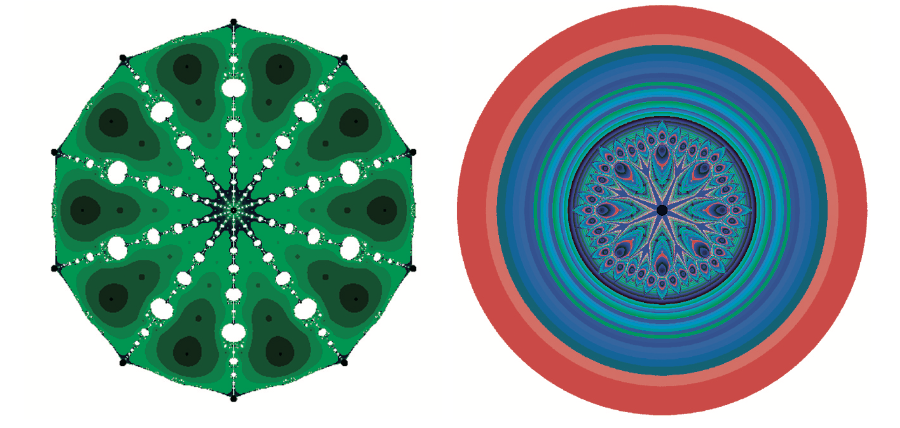
\includegraphics[width=0.7\textwidth]{fig1}
        \caption{Some examples from \citet{Kalantari_2008}}
    \end{figure}
\end{projectdefinition}

\begin{projectdesign}
	\begin{figure}[h]
		\centering
		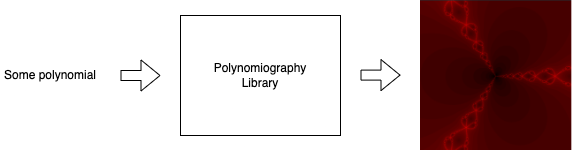
\includegraphics[width=1\textwidth]{fig2}
		\caption{Use Case 1}
	\end{figure}
\end{projectdesign}

\begin{projectdesign}
	\begin{figure}[h]
		\centering
		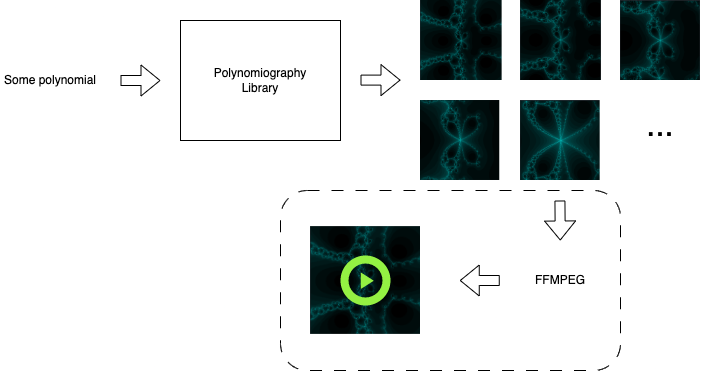
\includegraphics[width=1\textwidth]{fig3}
		\caption{Use Case 2}
	\end{figure}
\end{projectdesign}

\begin{contents}
        \frametitle{{\color{white} Project Design - Newton's Method}}
        \begin{itemize}
            \item 1 - Start with some $x$
            \item 2 - Iterate the following formula until the difference between $x_n$ and $x_{n+1}$ is less then some $\epsilon$
            \begin{center}
            \item \( x_{n+1} = x_n - \frac{f(x_n)}{f'(x_n)} \)
            \end{center}
            \item
            \item 3 - Return the approximated value [and iteration count]
        \end{itemize}
\end{contents}

\begin{contents}
        \frametitle{{\color{white} Project Design - Newton's Method - Examples}}
	\begin{figure}[h]
		\centering
		\caption{Polynomiography created using newton's method for $x^3 + 1$}
		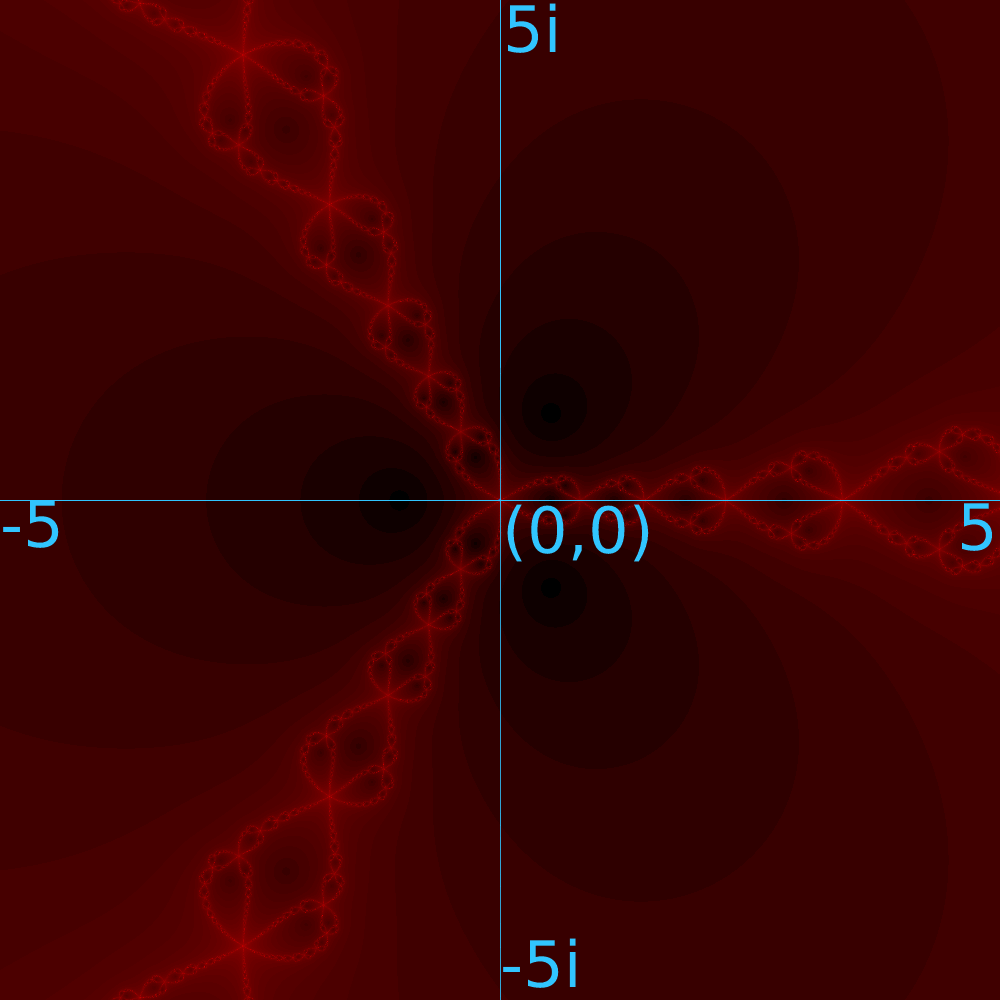
\includegraphics[width=0.6\textwidth]{fig4}
	\end{figure}
\end{contents}

\begin{contents}
        \frametitle{{\color{white} Project Design - Newton's Method - Examples}}
	\begin{figure}[h]
		\centering
		\caption{Polynomiography created using newton's method for $x^3 + 1$, multicolored}
		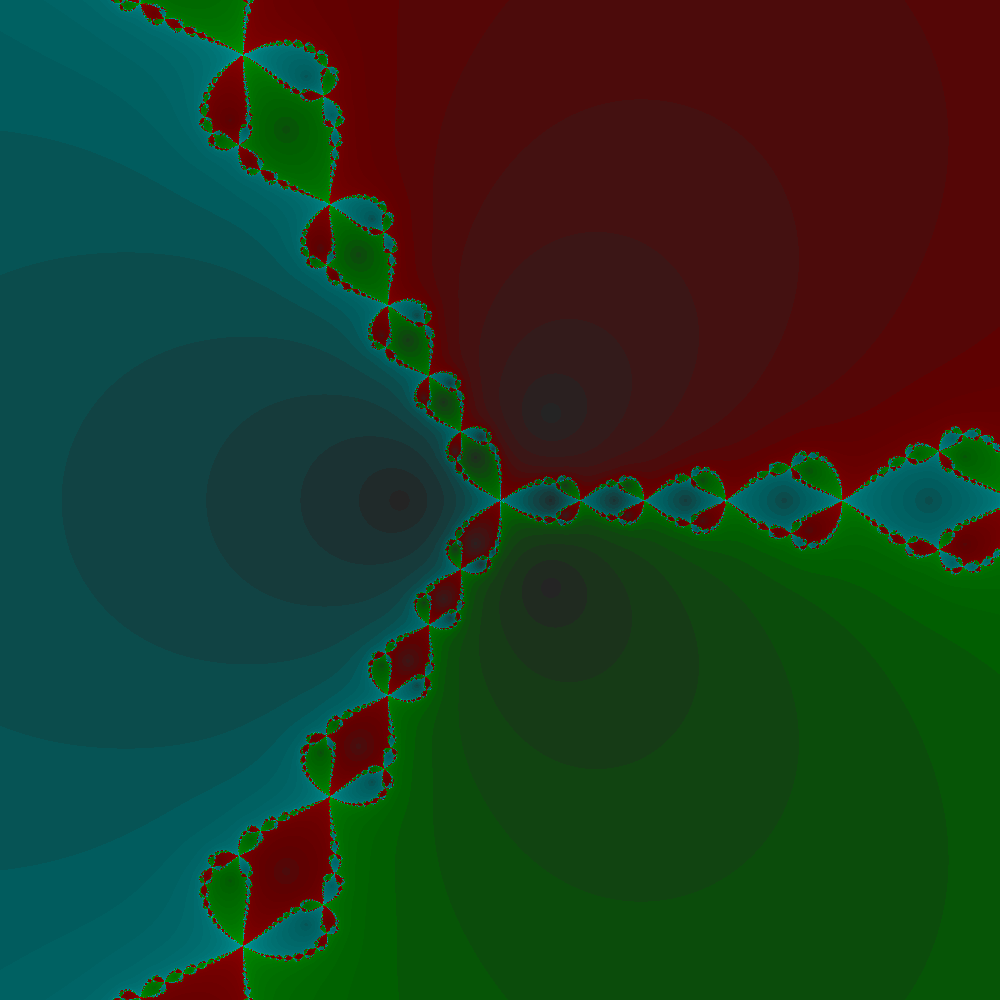
\includegraphics[width=0.6\textwidth]{fig5}
	\end{figure}
\end{contents}

\begin{projectrequirements}
\begin{itemize}
    \item[-] A complete python library that is ready to use for end-user
    \item[-] Code documentation
    \item[-] Simple GUI for demonstration
\end{itemize}
\end{projectrequirements}

\begin{contents}
	\frametitle{{\color{white} Timeline}}
	\begin{itemize}
	    \item \textbf{Apr 05: Preliminary Presentation}
	    \item Apr 05 - Apr 26: Research about previously implemented methods and root finding algorithms
	    \item Apr 27 - May 18: Implementation of the library
	    \item \textbf{May 17: 2$^{nd}$ Meeting}
	    \item May 18 - Jun 4: Implementation of GUI, updating documentation
            \item Jun 4 - Jun 18: Preparing the final draft of the report and trailer
	    \item \textbf{Jun 18: Report & Trailer Submissions}
	    \item \textbf{Jun 21: Final Presentation}
	    \item \textbf{Jun 22: Demo}
	\end{itemize}
\end{contents}

\begin{projectsuccess}
    \begin{itemize}[leftmargin=*]
        \item[-] At least 3 different methods that gives different result for the same polynomial
        \item[-] 
        \item[-] 
    \end{itemize}
\end{projectsuccess}

\begin{projectreferences}
    \footnotesize
\end{projectreferences}

\end{document}